\chapter{The \lhcb\ experiment}
\label{chap:intro:lhcb}

The \lhcb\ experiment~\cite{Alves:2008zz,Aaij:2014jba} comprises a 
collaboration of around one thousand scientists and engineers, and a particle 
detector situated at point 8 of the \cern\ \ac{LHC}.
The general goal of the experiment is to explore the area of heavy flavour 
physics, that is the interactions of charm and beauty quarks and the hadrons 
that contain them.
In particular, \lhcb\ aims to make, and already has made some of, the most 
precise measurements of heavy flavour properties to date, as well as to 
discover decays and particles that were not observed by previous experiments.
Heavy flavour has a rich phenomenology: neutral particles can oscillate between 
their matter and antimatter states in flight, such as $\PBds \leftrightarrow 
\APBds$ and $\PDzero \leftrightarrow 
\APDzero$~\cite{Abulencia:2006ze,Aaij:2012nva}; bound states of four or five 
quarks can form~\cite{Aaij:2014jqa,Aaij:2015tga}; they exhibit distinct 
matter-antimatter 
asymmetries~\cite{Aubert:2001nu,Abe:2001xe,Aaij:2012kz,Aaij:2013iua,Aaij:2016cla}; 
and their rare decays can be precisely predicated by the 
\ac{SM}~\cite{CMS:2014xfa,Aaij:2015oid}, as such being very sensitive to 
contributions from new theories..
With this, the \lhcb\ detector must be flexible enough to accommodate a wide 
physics programme. yet powerful enough to discriminate against the large 
backgrounds characteristic of a \pp\ collision environment.
This \namecref{chap:intro:lhcb} will link the properties of heavy flavour 
decays with the requirements imposed on the detector if these properties are to 
be studied.

At the \ac{LHC}, heavy flavour quarks are primarily produced through 
gluon-gluon fusion, illustrated in 
\cref{fig:intro:lhcb:hf_production:gg_fusion}.
With this mechanism, \bbbar\ and \ccbar\ pairs are predominantly produced in 
the forward region, at low angles to the beam, as shown in 
\cref{fig:intro:lhcb:hf_production:bbbar_angles}
To exploit this, the \lhcb\ detector is instrumented in the pseudorapidity 
region $2 < \Eta < 5$.
Particles produced in this region are highly boosted in the laboratory frame, 
and so given the lifetimes of the weakly decay heavy hadrons, of order of 
$0.1$--$\SI{1}{\pico\second}$~\cite{PDG2014}, they can fly several millimetres 
before decaying.
With a sufficiently sensitive detector, such secondary vertices can be 
spatially distinguish from the primary proton-proton interaction vertices, 
providing a powerful discriminant between signal and background.
A good secondary vertex resolution also allows for a good decay time 
resolution, which is necessary for measuring the fast oscillations of \PBds\ 
and \PDzero mesons, and for measuring any possible decay time asymmetries.
In addition, the large displacement of the decay vertices with respect to the 
\ac{PV} causes the particles produced at the vertex to have a high \ac{IP}, 
defined in \cref{fig:intro:lhcb:vertexing} as the smallest transverse distance 
from the particle trajectory to the \ac{PV}.
A sufficient experimental resolution on the \ac{IP} allows for additional 
discrimination between random tracks in the event and those from heavy flavour 
decays.
The precise reconstruction of primary and secondary vertices requires a precise 
tracking system, particularly so close to the \pp\ interaction region, and so 
the detector design is highly optimised for tracking performance.
The tracking system will be described in 
\cref{chap:intro:lhcb:detector:tracking}.

The properties of heavy flavour hadrons, such as their masses and lifetimes, 
can be inferred by reconstructing the four-momenta of their decay products, and 
so most analyses at \lhcb\ aim to fully reconstruct the decays of beauty and 
charm hadrons, such as $\decay{\PBz}{\PKplus\PKminus}$, 
$\decay{\PBs}{\PDspm\PKmp}$ with $\decay{\PDsplus}{\PKminus\PKplus\Ppiplus}$, 
$\decay{\PLambdab}{\PJpsi\Pproton\PKminus}$ with 
$\decay{\PJpsi}{\Pmuon\APmuon}$, and $\decay{\PDz}{\PKplus\Ppiminus}$.
It is important to note that specific final states offer higher sensitivities 
to physics observables than others, and so it is crucial for \lhcb\ to be able 
to distinguish between different particle species.
For example, the decay $\decay{\PDz}{\PKplus\Ppiminus}$ is of the order of one 
thousand times less likely than the decay $\decay{\PDz}{\PKminus\Ppiminus}$, 
and so a poor \ac{PID} performance would result in a search for the 
$\PKplus\Ppiminus$ final state being dominated by $\PKminus\Ppiplus$ 
`background'.
In general, misidentification cannot be excluded completely, and so in addition 
a high momentum resolution is required to be able to distinguish between 
different final states in the parent mass spectrum.

An example of the power of, and necessity for, good particle identification and 
momentum resolution is shown in \cref{fig:intro:lhcb:pid_power}.
Here, the signal decay is \decay{\PBzero}{\pimpip}, and the distributions are 
the two-body invariant mass before \ac{PID} requirements are made on the 
tracks~(\ref{fig:intro:lhcb:pid_power:pre}) and 
after~(\ref{fig:intro:lhcb:pid_power:post}).
As can be seen, before the requirements the distribution is dominated by other 
two-body \PBzero, \PBs, and \PLambdab\ decays, whereas after the selection the 
backgrounds are almost entirely removed.
The presence of such backgrounds significantly increases the complexity of an 
analysis and can reduce the precision of the measurement.

In the following, the construction of the detector will be described, as 
motivated by the physics goals of the collaboration and the properties of heavy 
flavour outlined above.

\begin{figure}
  \begin{subfigure}[b]{0.4\textwidth}
    \centering
    \feynmandiagram [large, horizontal=a to b] {%
  i1 [particle=\(\Pgluon\)] -- [gluon] a -- [gluon] i2 [particle=\(\Pgluon\)],
  a -- [gluon, edge label=\(\Pgluon\)] b,
  f1 [particle=\(\APquark\)] -- [fermion] b -- [fermion] f2 [particle=\(\Pquark\)],
};

    \caption{Quark pair production}
    \label{fig:intro:lhcb:hf_production:gg_fusion}
  \end{subfigure}
  \begin{subfigure}[b]{0.6\textwidth}
    \begin{tikzpicture}
  \node[anchor=south west, inner sep=0] (image) at (0, 0) {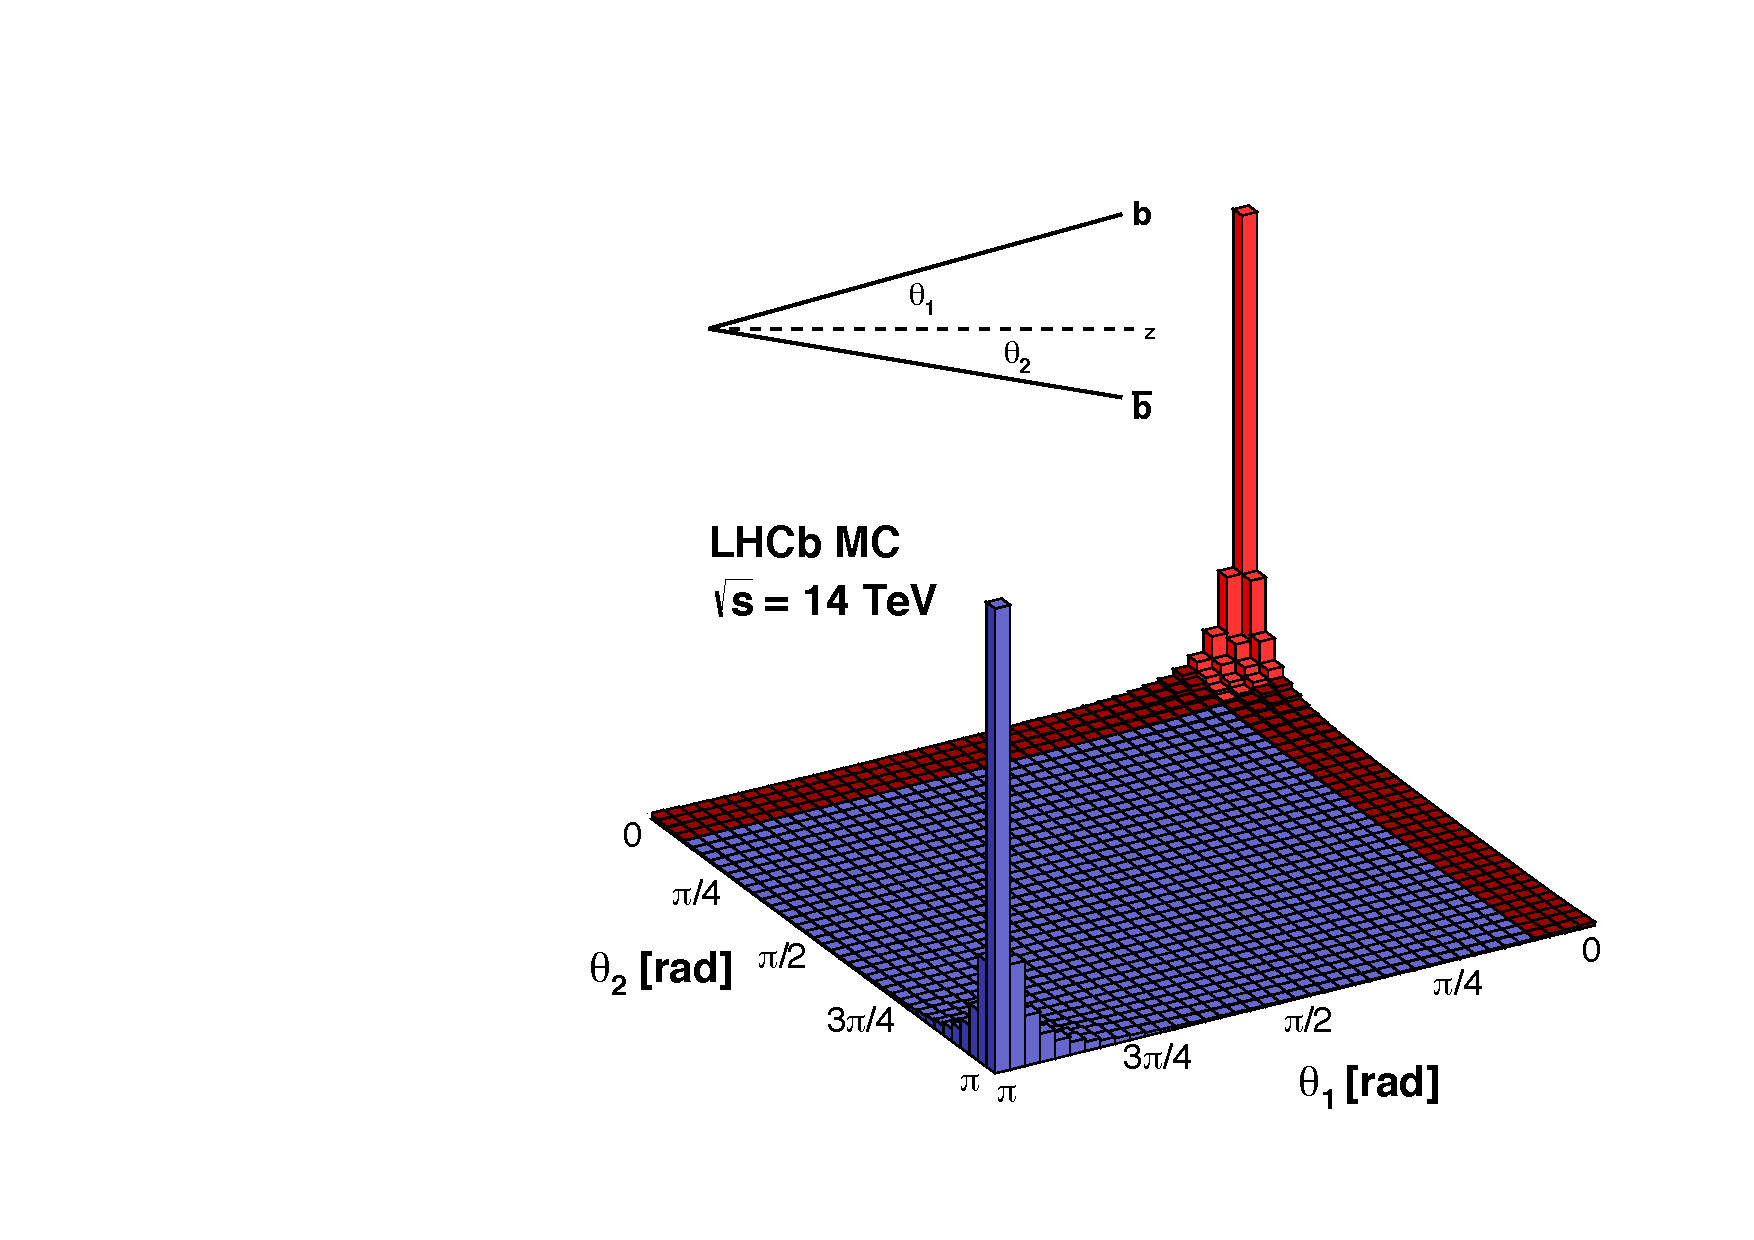
\includegraphics[width=\textwidth]{introduction/bbbar_production_angles}};
  \begin{scope}[x={(image.south east)}, y={(image.north west)}]
    % Grid to help find coordinates on the image
    % \draw[step=0.02, gray, very thin] (0, 0) grid (1, 1);
    % Box to cover axis labels
    \path[fill=white] (0.02, 0.16) rectangle (0.18, 0.22) node [pos=0.5] {\footnotesize$\theta_{1}$};
    \path[fill=white] (0.64, 0.06) rectangle (0.78, 0.12) node [pos=0.5] {\footnotesize$\theta_{2}$};
    % Box to cover angle definitions
    \path[fill=white] (0.14, 0.66) rectangle (0.54, 0.88);
    % Box to cover 'LHCb MC' label
    \path[fill=white] (0.14, 0.48) rectangle (0.36, 0.58);
  \end{scope}
\end{tikzpicture}

    \caption{$\Pbottom\APbottom$ production distribution}
    \label{fig:intro:lhcb:hf_production:bbbar_angles}
  \end{subfigure}
  \caption{%
    Feynman diagram of quark pair production via gluon-gluon fusion 
    (\subref*{fig:intro:lhcb:hf_production:gg_fusion}), and a simulation of the 
    angular distribution of \bbbar\ production at the \ac{LHC} at $\sqrt{s} = 
    \SI{13}{\TeV}$ (\subref*{fig:intro:lhcb:hf_production:bbbar_angles}).
  }
  \label{fig:intro:lhcb:hf_production}
\end{figure}

\begin{figure}
  \begin{subfigure}[b]{0.5\textwidth}
    \centering
    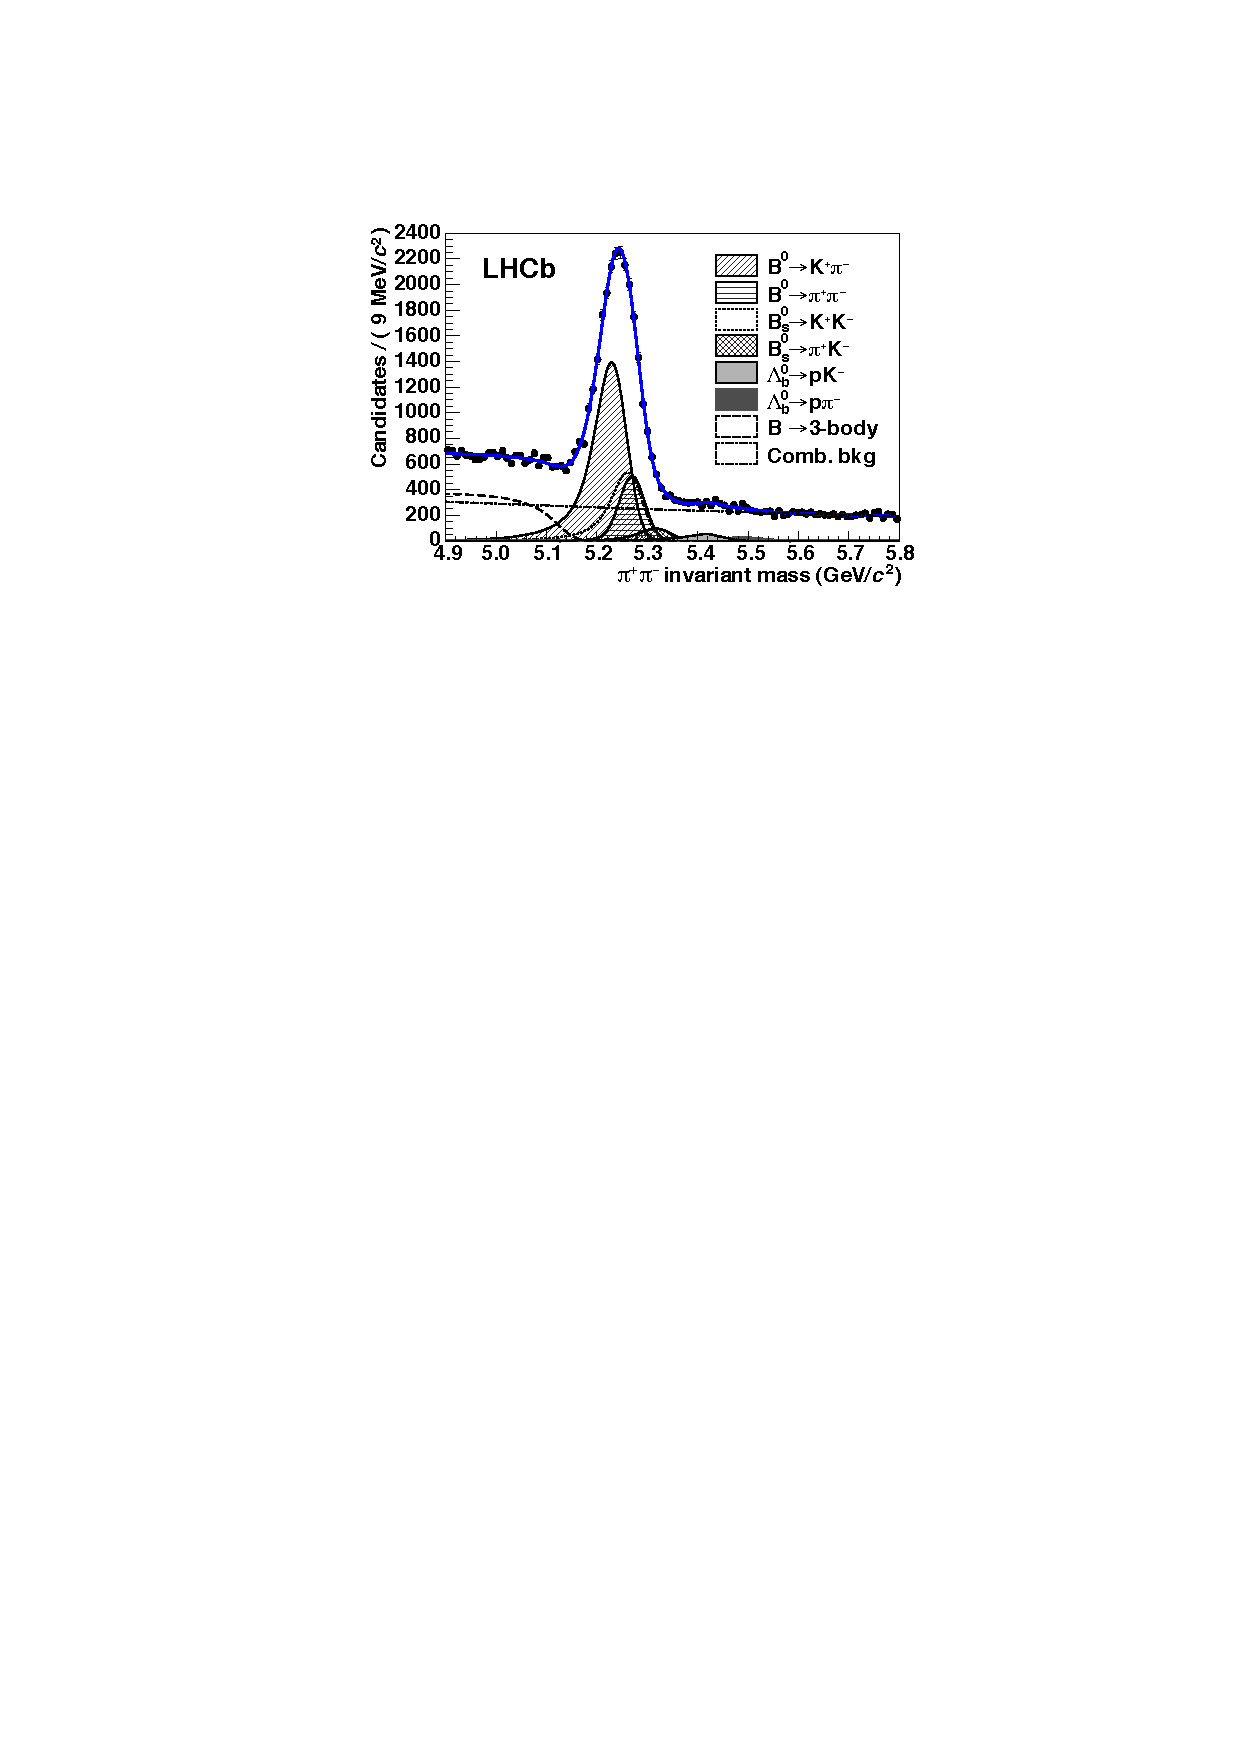
\includegraphics[width=\textwidth]{introduction/B2pipi_pre_pid}
    \caption{Before \ac{PID} requirements}
    \label{fig:intro:lhcb:pid_power:pre}
  \end{subfigure}
  \begin{subfigure}[b]{0.5\textwidth}
    \centering
    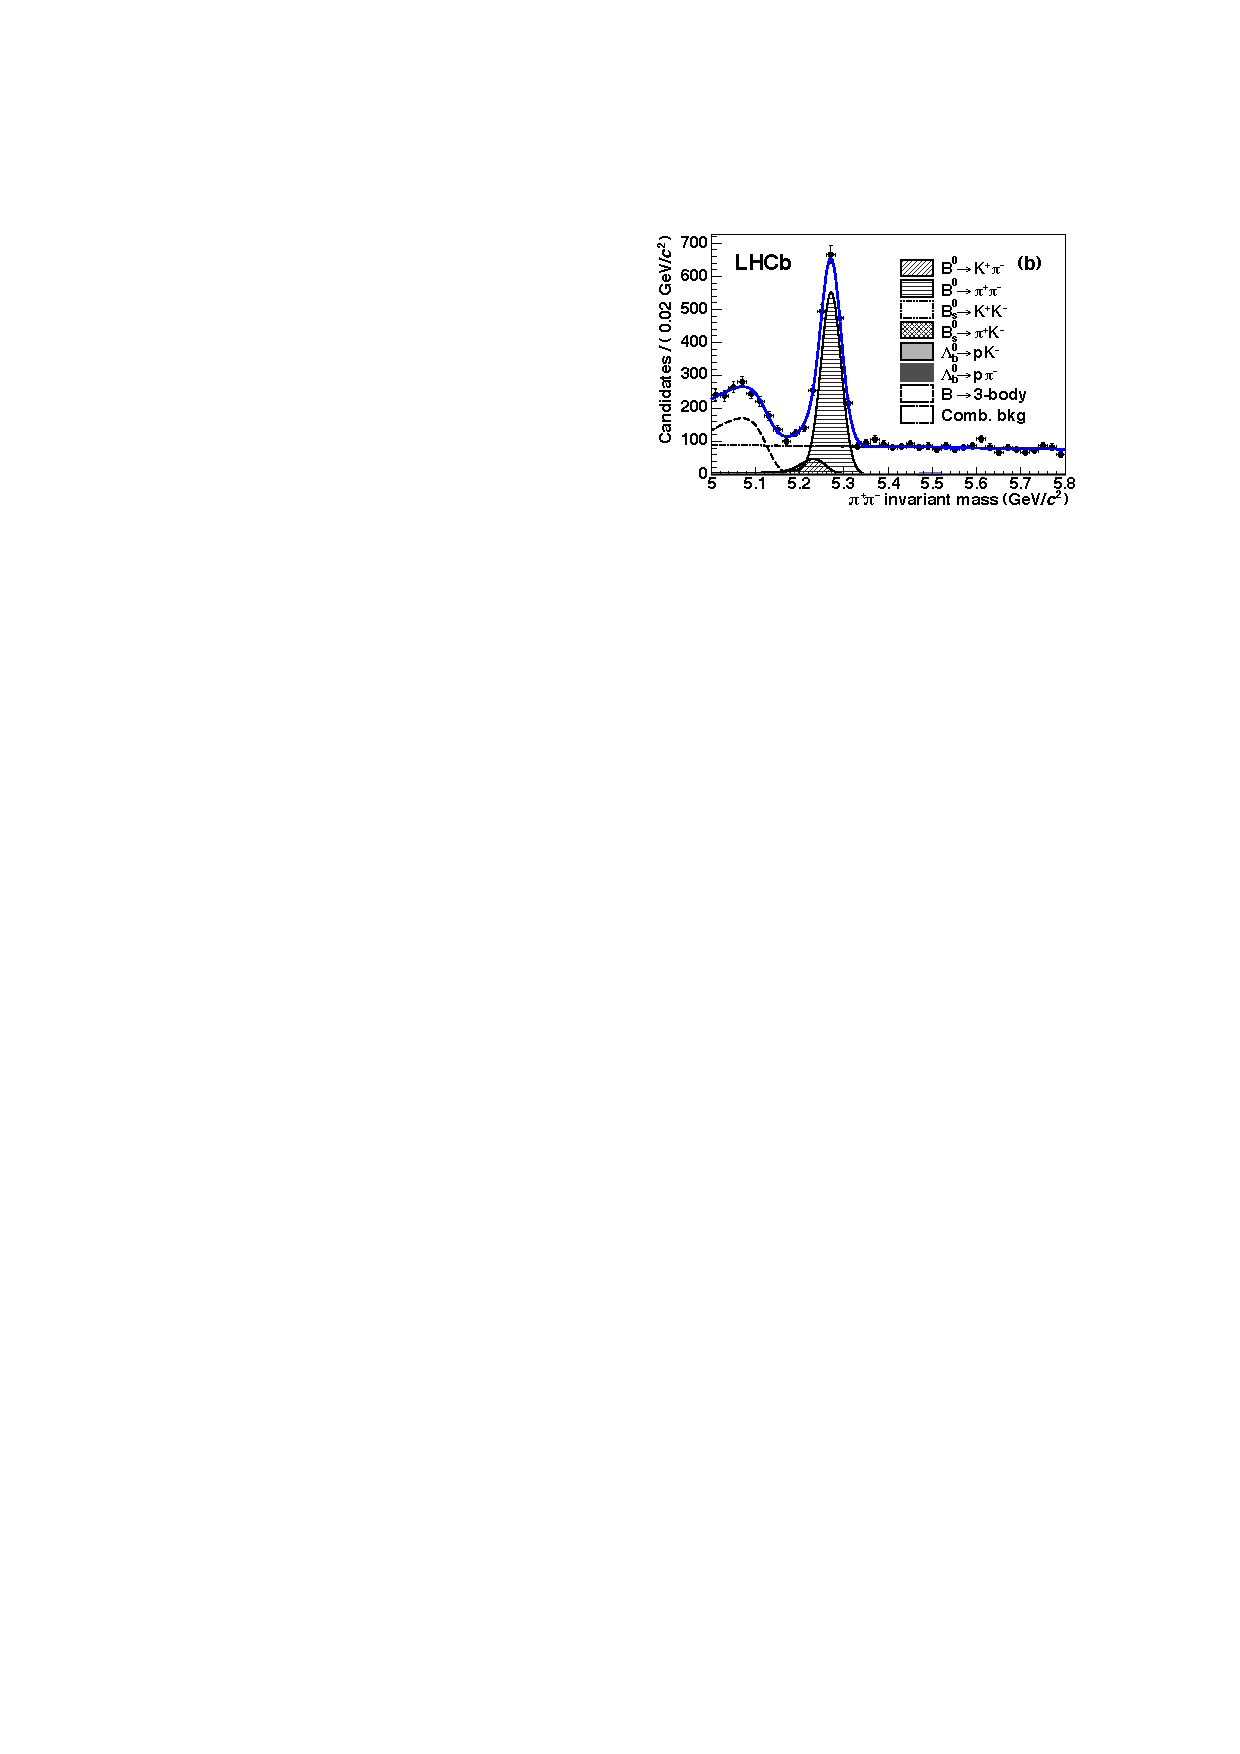
\includegraphics[width=\textwidth]{introduction/B2pipi_post_pid}
    \caption{After \ac{PID} requirements}
    \label{fig:intro:lhcb:pid_power:post}
  \end{subfigure}
  \caption{%
    Two-body invariant mass spectrum, under the $\pimpip$ hypothesis, 
    before~(\subref*{fig:intro:lhcb:pid_power:pre}) and 
    after~(\subref*{fig:intro:lhcb:pid_power:post}) \ac{PID} 
    requirements~\cite{Aaij:2012as}.
    The contribution from the signal decay is hatched with horizontal lines.
  }
  \label{fig:intro:lhcb:pid_power}
\end{figure}

\section{Detector}
\label{chap:intro:lhcb:detector}

Within the \lhcb\ experiment, the co-ordinate system is defined such that the 
$z$-axis is aligned along the beam direction, increasing in the clockwise 
direction along the \ac{LHC} ring; the $y$-axis is aligned with gravity, 
increasing away from the Earth's surface; and the $x$-axis, defined as $x = y 
\times z$, is then increasing away from the centre of the accelerator.
In this \namecref{chap:intro:lhcb:detector}, and in all that follows, this 
coordinate system will be used.

A schematic of the detector is given in \cref{fig:intro:lhcb:detector}.
Its forward geometry is evident, being instrumented in the region $2 < \Eta < 
5$.
A dipole magnet with an integrated field strength of \SI{4}{\tesla\metre} bends 
charged particle trajectories in the $xz$ plane, with its polarity being 
switched periodically during data-taking.
Charged particle trajectories are recorded by the tracking system.
This is composed of a vertex detector centred around the proton-proton 
interaction region, three planes of tracking stations before the magnet, and 
three planes after.
Immediately downstream of the vertex detector, increasing is $z$, is the first 
of two \ac{RICH} detectors, each used for particle identification, the second 
of which is after the tracking stations downstream of the magnet.
After this, a calorimetry system is in place to identify neutral particles such 
as the \Ppizero\ and the photon, as well as to measure their energy and that of 
the charged particles.
Finally, a muon system is installed after the calorimeters, which is used for 
muon identification.

The data recorded by the detector is selected in real time by a hardware 
trigger, after which a two-stage software trigger performs an event 
reconstruction.
There are not enough computing resources available to the experiment to record 
and analyse every proton-proton bunching crossing, and so the trigger is as 
important to achieving the physics goals of the collaboration as the detector.
The trigger responsible for deciding which crossings should be kept and which 
should be discarded.
The design of the detector and the trigger were made in consideration of one 
another.

Each sub-detector shall now be described in turn, followed by a description of 
the trigger system.
The descriptions will relate to the detector and its performance during 
\runone, and shall be followed by a Section on the upgrades performed during 
\ac{LS1}.

\begin{figure}
  \centering
  \begin{tikzpicture}
  % Use trim and crop to remove some of the white space around the image
  \node[anchor=south west, inner sep=0] (image) at (0, 0) {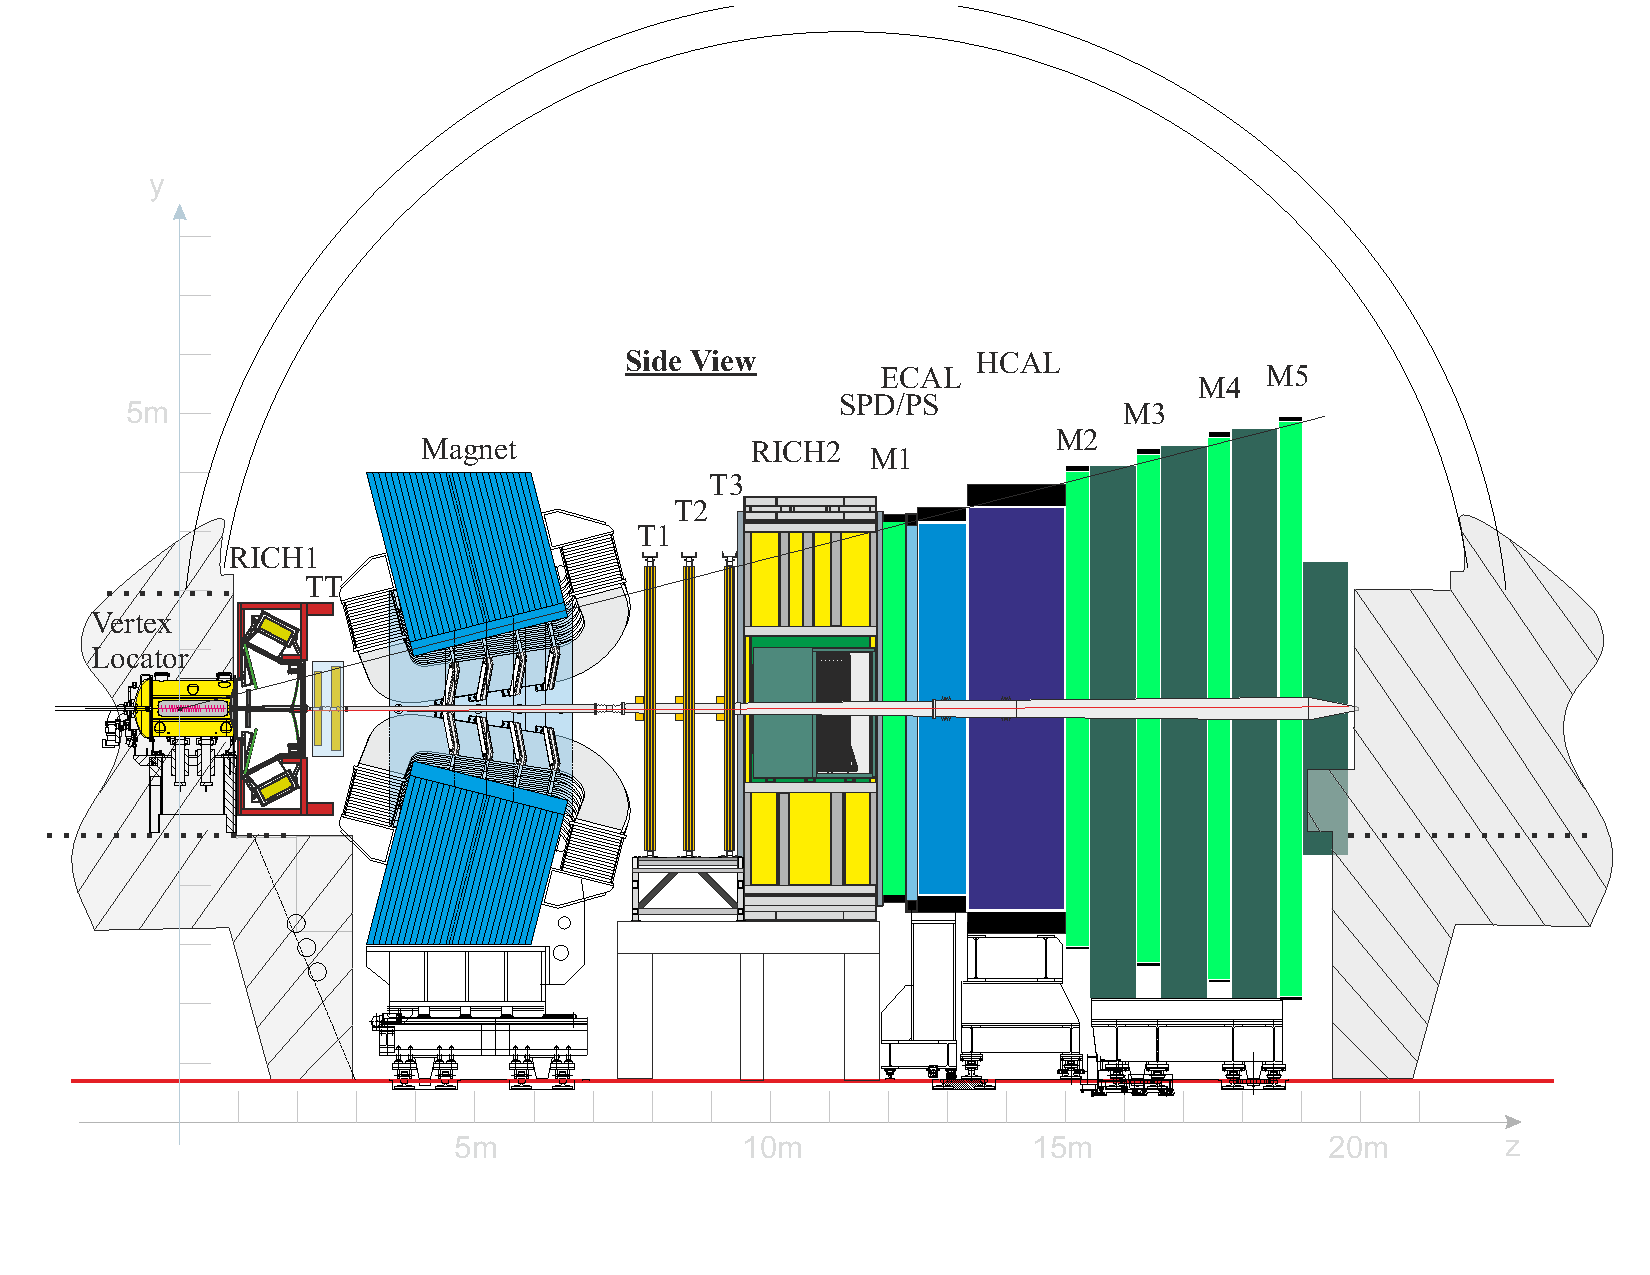
\includegraphics[width=\textwidth, trim={1cm 1.7cm 0.5cm 3cm}, clip]{introduction/lhcb_detector}};
  \begin{scope}[x={(image.south east)}, y={(image.north west)}]
    % Grid to help find coordinates on the image
    % \draw[step=0.02, gray, very thin] (0, 0) grid (1, 1);
    % Box to cover "Side View" label
    \path[fill=white] (0.36, 0.78) rectangle (0.46, 0.84);
  \end{scope}
\end{tikzpicture}

  \caption{%
    A schematic of the \lhcb\ detector.
    In this Figure, the $z$-axis, labelled, increases from left to right, the 
    $y$-axis, also labelled, increases from bottom to top, and the $x$-axis 
    increases into the page.
  }
  \label{fig:intro:lhcb:detector}
\end{figure}

\subsection{Tracking}
\label{chap:intro:lhcb:detector:tracking}

Charged particle trajectories are reconstructed as tracks using hits deposited 
in the tracking system.
This comprises the vertex locator~(\velo) centred around the \pp\ interaction 
region, the Tracker Turicensis~(\ttracker) before the magnet, and the 
T-stations after the magnet.
In \runone, the tracking system achieved a momentum resolution 
$\unc{\ptot}/\ptot$ from \SI{0.5}{\percent} at $\ptot = \SI{5}{\GeVc}$ to 
\SI{0.8}{\percent} at \SI{100}{\GeVc}, and a track \acl{IP} resolution varying 
from around \SI{70}{\micro\metre} for tracks with a low \pT\ to 
\SI{20}{\micro\metre} at high \pT.

The \velo\ is an extremely precise silicon strip detector, whose active 
elements come as close as \SI{8}{\milli\metre} away from the \ac{LHC} beams.
Two sets of 24 silicon modules are arranged either side of the beam, each of 
which measures particle hits in $r$ and $\phi$ coordinates.
Charged particles traversing the active silicon can ionise the material, 
creating electron-hole pairs that drift towards the electrodes, registering a 
hit as an electrical signal.
The magnetic field strength inside the \velo\ is approximated to be zero, and 
so track segments are reconstructed as straight lines using the hits in the 
sensors.
So-called long tracks, the track type used for the majority of physics 
analyses, are created by combining \velo\ segments with hits in the T-stations 
after the magnet.

The three T-stations, T1--3, each comprise a silicon strip detector close to 
the beam pipe~(the \itracker) and a drift-tube detector in the outer 
regions~(the \otracker).
The \itracker\ has a finer spatial resolution than the \otracker, and covers a 
small area around the beam where the particle multiplicities are particularly 
high.
The \otracker\ covers an area of approximately \SI{30}{\metre\squared}, about 8 
times greater than that covered by the \itracker.
Ionising particles free electrons from the gas molecules within the tubes, 
which are detected by anode wires and registered as hits.
The point of ionisation within the wire is determined by measuring the electron 
drift time, improving the track momentum resolution.
This is further improved by adding the hits detected in the \ttracker, upstream 
of the T-stations.
The \ttracker\ is a silicon strip detector of the same technology as the 
\itracker, with the three stations covering a total area of around 
\SI{8}{\metre\squared}.

The tracking efficiency, the fraction of real tracks that are formed given that 
enough hits were deposited to form one, is measured using a tag-and-probe 
technique with \JpsiTomumu\ decays, which will be explained in more detail in 
\cref{chap:prod:effs:tracking}.
The average tracking efficiency is measured to be above 
\SI{95}{\percent}~\cite{Aaij:2014pwa}.
The formation of tracks assumes that the tracker system is perfectly aligned, 
but the positions of the various stations can change with time.
To compensate for this effect, alignment constants are computed periodically 
and used in the reconstruction software.
The effect of an improved alignment is illustrated in 
\cref{fig:intro:lhcb:alignment}, where the $\Pmuon\APmuon$ mass resolution 
improves from \SI{92}{\MeVcc} with an initial alignment to \SI{49}{\MeVcc} with 
an improved one, which more accurately reflects the state of the 
detector~\cite{Dujany:082010}.
Without the improved alignment, it is harder to distinguish three distinct 
resonant states.

\begin{figure}
  \centering
  % Draw perpendicular markers at line intersections
% http://tex.stackexchange.com/a/21759/45857
\tikzset{
  right angle quadrant/.code={
    \pgfmathsetmacro\quadranta{{1,1,-1,-1}[#1-1]}     % Arrays for selecting quadrant
    \pgfmathsetmacro\quadrantb{{1,-1,-1,1}[#1-1]}},
  right angle quadrant=1, % Make sure it is set, even if not called explicitly
  right angle length/.code={\def\rightanglelength{#1}},   % Length of symbol
  right angle length=2ex, % Make sure it is set...
  right angle symbol/.style n args={3}{
    insert path={
      let \p0 = ($(#1)!(#3)!(#2)$) in     % Intersection
      let \p1 = ($(\p0)!\quadranta*\rightanglelength!(#3)$), % Point on base line
      \p2 = ($(\p0)!\quadrantb*\rightanglelength!(#2)$) in % Point on perpendicular line
      let \p3 = ($(\p1)+(\p2)-(\p0)$) in  % Corner point of symbol
      (\p1) -- (\p3) -- (\p2)
    }
  }
}
\begin{tikzpicture}[
  x=2cm,
  y=2cm,
  axis/.style={very thick,->,gray},
  beam/.style={very thick,->,gray},
  scale=1.5,
  thick
  ]
  % Origin
  \coordinate (O) at (0, 0);
  % B decay vertex
  \coordinate (Bvtx) at (1, 0.5);
  % Offset of muon arrows, with respect to Bvtx
  \coordinate(mumoffset) at (0.3, 0.4);
  \coordinate(mupoffset) at (0.6, -0.2);
  % Compute the coordinates of the ends of the muon lines
  \coordinate (mum) at ($(Bvtx) + (mumoffset)$);
  \coordinate (mup) at ($(Bvtx) + (mupoffset)$);

  % Coordinate axes
  \draw[axis] (-0.6, -0.5) -- +(0.2, 0) node [below] {$z$};
  \draw[axis] (-0.6, -0.5) -- +(0, 0.2) node [left] {$y$};

  \draw[beam] (-1.0, 0) -- (-0.1, 0) node [below, at start] {$p$};
  \draw[beam] (1.5, 0) -- (0.1, 0) node [below, at start] {$p$};

  % D meson
  \draw[dashed, color=gray, text=black] (O) -- (Bvtx) node [above, pos=0.5] {\PDz};
  % Negative child
  \draw[->] (Bvtx) -- (mum) node [above] {\PKminus};
  \draw[dotted] (Bvtx) -- ($(Bvtx) - 3*(mumoffset)$) node [name=mumend] {};
  % Positive child
  \draw[->] (Bvtx) -- (mup) node [below] {\Ppiplus};
  \draw[dotted] (Bvtx) -- ($(Bvtx) - 2*(mupoffset)$) node [name=mupend] {};

  % Primary vertex
  \node[star,star points=10,draw=orange!50,fill=orange!20,inner sep=0pt,minimum size=0.4cm] at (O) {};

  % Negative muon IP
  \draw[right angle length=1mm, right angle symbol={Bvtx}{mumend}{O}] ($(Bvtx)!(O)!(mumend)$) -- (O) node [pos=0.2, left] {$\text{IP}_{\PKminus}$};
  % Positive muon IP
  \draw[right angle length=1mm, right angle symbol={Bvtx}{mupend}{O}] ($(Bvtx)!(O)!(mupend)$) -- (O) node [midway, left] {$\text{IP}_{\Ppiplus}$};
\end{tikzpicture}

  \caption{%
    Illustration of vertexing, showing a \PDz meson decaying in flight to a 
    kaon and a pion.
    The kaon and pion are reconstructed as tracks, and then the \PDzero decay 
    vertex is inferred from the point of closest approach of the two tracks.
    The minimum transverse distance the tracks make when extrapolated back 
    towards the primary proton-proton vertex, the \acf{IP}, is shown.
  }
  \label{fig:intro:lhcb:vertexing}
\end{figure}

\begin{figure}
  \begin{subfigure}{0.5\textwidth}
    \centering
    \begin{tikzpicture}
  \node[anchor=south west, inner sep=0] (image) at (0, 0) {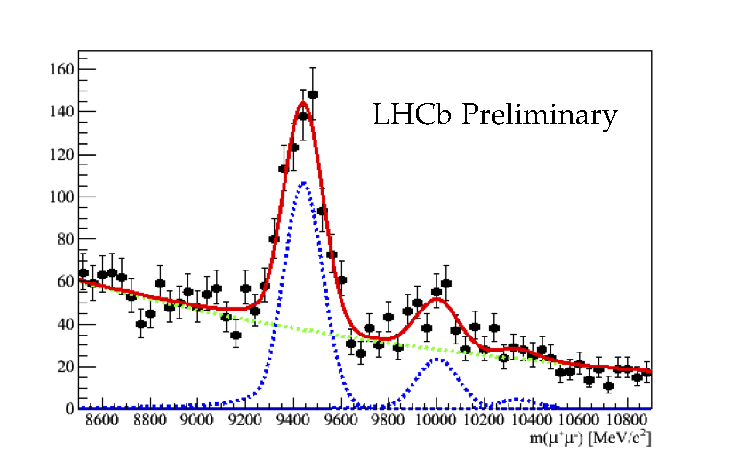
\includegraphics[width=\textwidth]{introduction/mumu_pre_alignment}};
  \begin{scope}[x={(image.south east)}, y={(image.north west)}]
    % Grid to help find coordinates on the image
    % \draw[step=0.05, gray, very thin] (0, 0) grid (1, 1);
    % Box to cover 'LHCb preliminary' label
    \path[fill=white] (0.5, 0.7) rectangle (0.85, 0.8);
  \end{scope}
\end{tikzpicture}

    \caption{Before}
    \label{fig:intro:lhcb:alignment:pre}
  \end{subfigure}
  \begin{subfigure}{0.5\textwidth}
    \centering
    \begin{tikzpicture}
  \node[anchor=south west, inner sep=0] (image) at (0, 0) {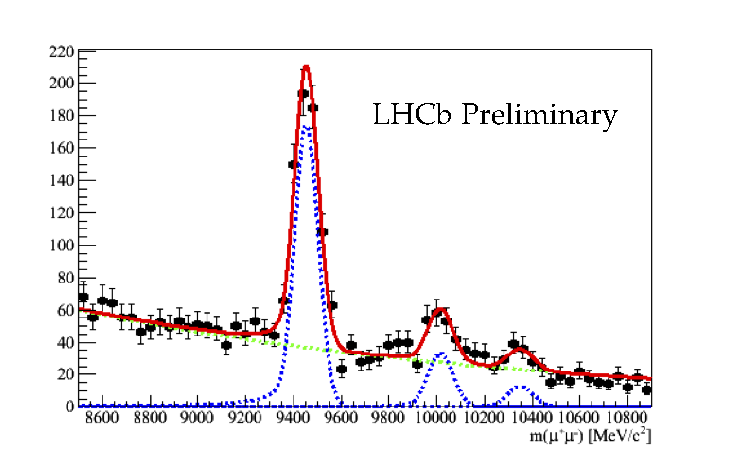
\includegraphics[width=\textwidth]{introduction/mumu_post_alignment}};
  \begin{scope}[x={(image.south east)}, y={(image.north west)}]
    % Grid to help find coordinates on the image
    % \draw[step=0.05, gray, very thin] (0, 0) grid (1, 1);
    % Box to cover 'LHCb preliminary' label
    \path[fill=white] (0.5, 0.7) rectangle (0.85, 0.8);
  \end{scope}
\end{tikzpicture}

    \caption{After}
    \label{fig:intro:lhcb:alignment:post}
  \end{subfigure}
  \caption{%
    Invariant mass distribution of di-muon candidates in the region of the 
    first three \PUpsilon resonances~\cite{Dujany:082010}.
    The left plot~(\subref*{fig:intro:lhcb:alignment:pre}) shows the data 
    reconstructed with a preliminary alignment, whilst the right 
    plot~(\subref*{fig:intro:lhcb:alignment:post}) shows the result of a 
    reconstruction performed with a revised alignment.
    The di-muon mass resolution improves from \SI{92}{\MeVcc} to 
    \SI{49}{\MeVcc}.
  }
  \label{fig:intro:lhcb:alignment}
\end{figure}

\subsection{Particle identification}
\label{chap:intro:lhcb:detector:pid}

In order to compute the invariant mass of a decay vertex, the mass of the 
tracks forming that vertex must be known.
As each long-lived charged particle has a unique mass, the mass measurement 
assigns an identity to that track, in the process of \acf{PID}.
Through the momentum-velocity relation, the mass of a particle can be 
determined by combining the momentum measurement from the tracking system with 
a velocity measurement, which is performed by the \rich\ detectors.

Tracks created by pions, kaons, and protons are identified using the response 
of two \acl{RICH} detectors: \richone\ located upstream of the magnet; and 
\richtwo\ located downstream.
They also provide electron and muon discrimination, albeit at a weaker level.
\richtwo\ has larger surface area than \richone\ but has a smaller angular 
acceptance, being designed to efficiently identify tracks with momenta in the 
range \SIrange{15}{100}{\GeVc} which largely occupy the low-$\theta$ region.
\richone\ is effective in the momentum range \SIrange{3}{60}{\GeVc}.
During \runone, \richone\ contained a mixture of aerogel and \ce{C4F10} gas, of 
which the former was removed before the start of \runtwo.
\richtwo\ contains \ce{CF4} gas mixed with a small amount of \ce{CO2} to quench 
scintillation light.

As charged particles travel through one of the `radiators', each of refractive 
index $n$, the particles emit Cherenkov radiation if they are travelling faster 
than the phase velocity of light of the radiator.
This light is emitted at an angle $\thetac$ to the particle trajectory, and is 
related to the speed of the particle as
\begin{equation}
  \cos{\thetac} = \frac{1}{n\beta},
\end{equation}
where $\beta = v/c$.
The refractive indices of the radiators are known and are controlled by 
monitoring the gas pressure and temperature over time.
By measuring \thetac\ the \rich\ detectors can provide velocity measurements of 
charged tracks, thereby identifying them.

The Cherenkov light cones are reflected outside of the \lhcb detector 
acceptance by spherical and plane mirrors onto planes of photon detector 
arrays.
The angle \thetac\ is related to the radius of the rings, and, for a given 
momentum particles, of different masses will produced smaller or larger rings.
\Cref{fig:intro:lhcb:cherenkov_angles} illustrates the Cherenkov angles emitted 
by different particle species as a function of particle momentum.
Separation between mass hypotheses is given by the difference between the 
angles, denoted on the $y$-axis.
Discrimination can also be provided by the lack of Cherenkov light if a track 
has a momentum between two momentum thresholds.
The Cherenkov angle resolution in \richone\ is around \SI{1.6}{\milli\radian}, 
and around \SI{0.66}{\milli\radian} in \richtwo.

In order to assign a particle mass hypothesis to a track, a maximum likelihood 
method is used~\cite{Forty:1998eqa}.
Initially, all reconstructed tracks are assumed to be pions, and the 
\emph{predicted} Cherenkov rings assuming this hypothesis set are projected 
onto the photo-detector planes within both \richone\ and \richtwo.
The value of the log-likelihood is computed by comparing the predicted number 
of photons within each photo-detector to that observed.
For each track, the mass hypothesis is then changed to each of (\Pe, \Pmu, 
\Ppi, \PK, \Pproton), the rings assuming the new global hypothesis set are 
projected, and the log-likelihood is re-computed.
The hypothesis giving the largest increase in the log-likelihood is recorded, 
and the track hypothesis is returned back to its original value.
After all individual track hypotheses have been trialled, the single hypothesis 
change that gave the largest increase in the log-likelihood is applied to the 
respective track.
This procedure is repeated until the log-likelihood no longer increases with 
any change in the hypothesis set.
The outputs of this method are the \ac{DLL} variables, with one value per track 
for each of the (\Pe, \Pmu, \PK, \Pproton) hypotheses.
Each \ac{DLL} variable is defined as the difference in the log-likelihood value 
when the track mass hypothesis is changed from the pion hypothesis to the one 
of the variable, for example \dllkpi.
The pion \dll\ value is then zero by definition.

\begin{figure}
  \centering
  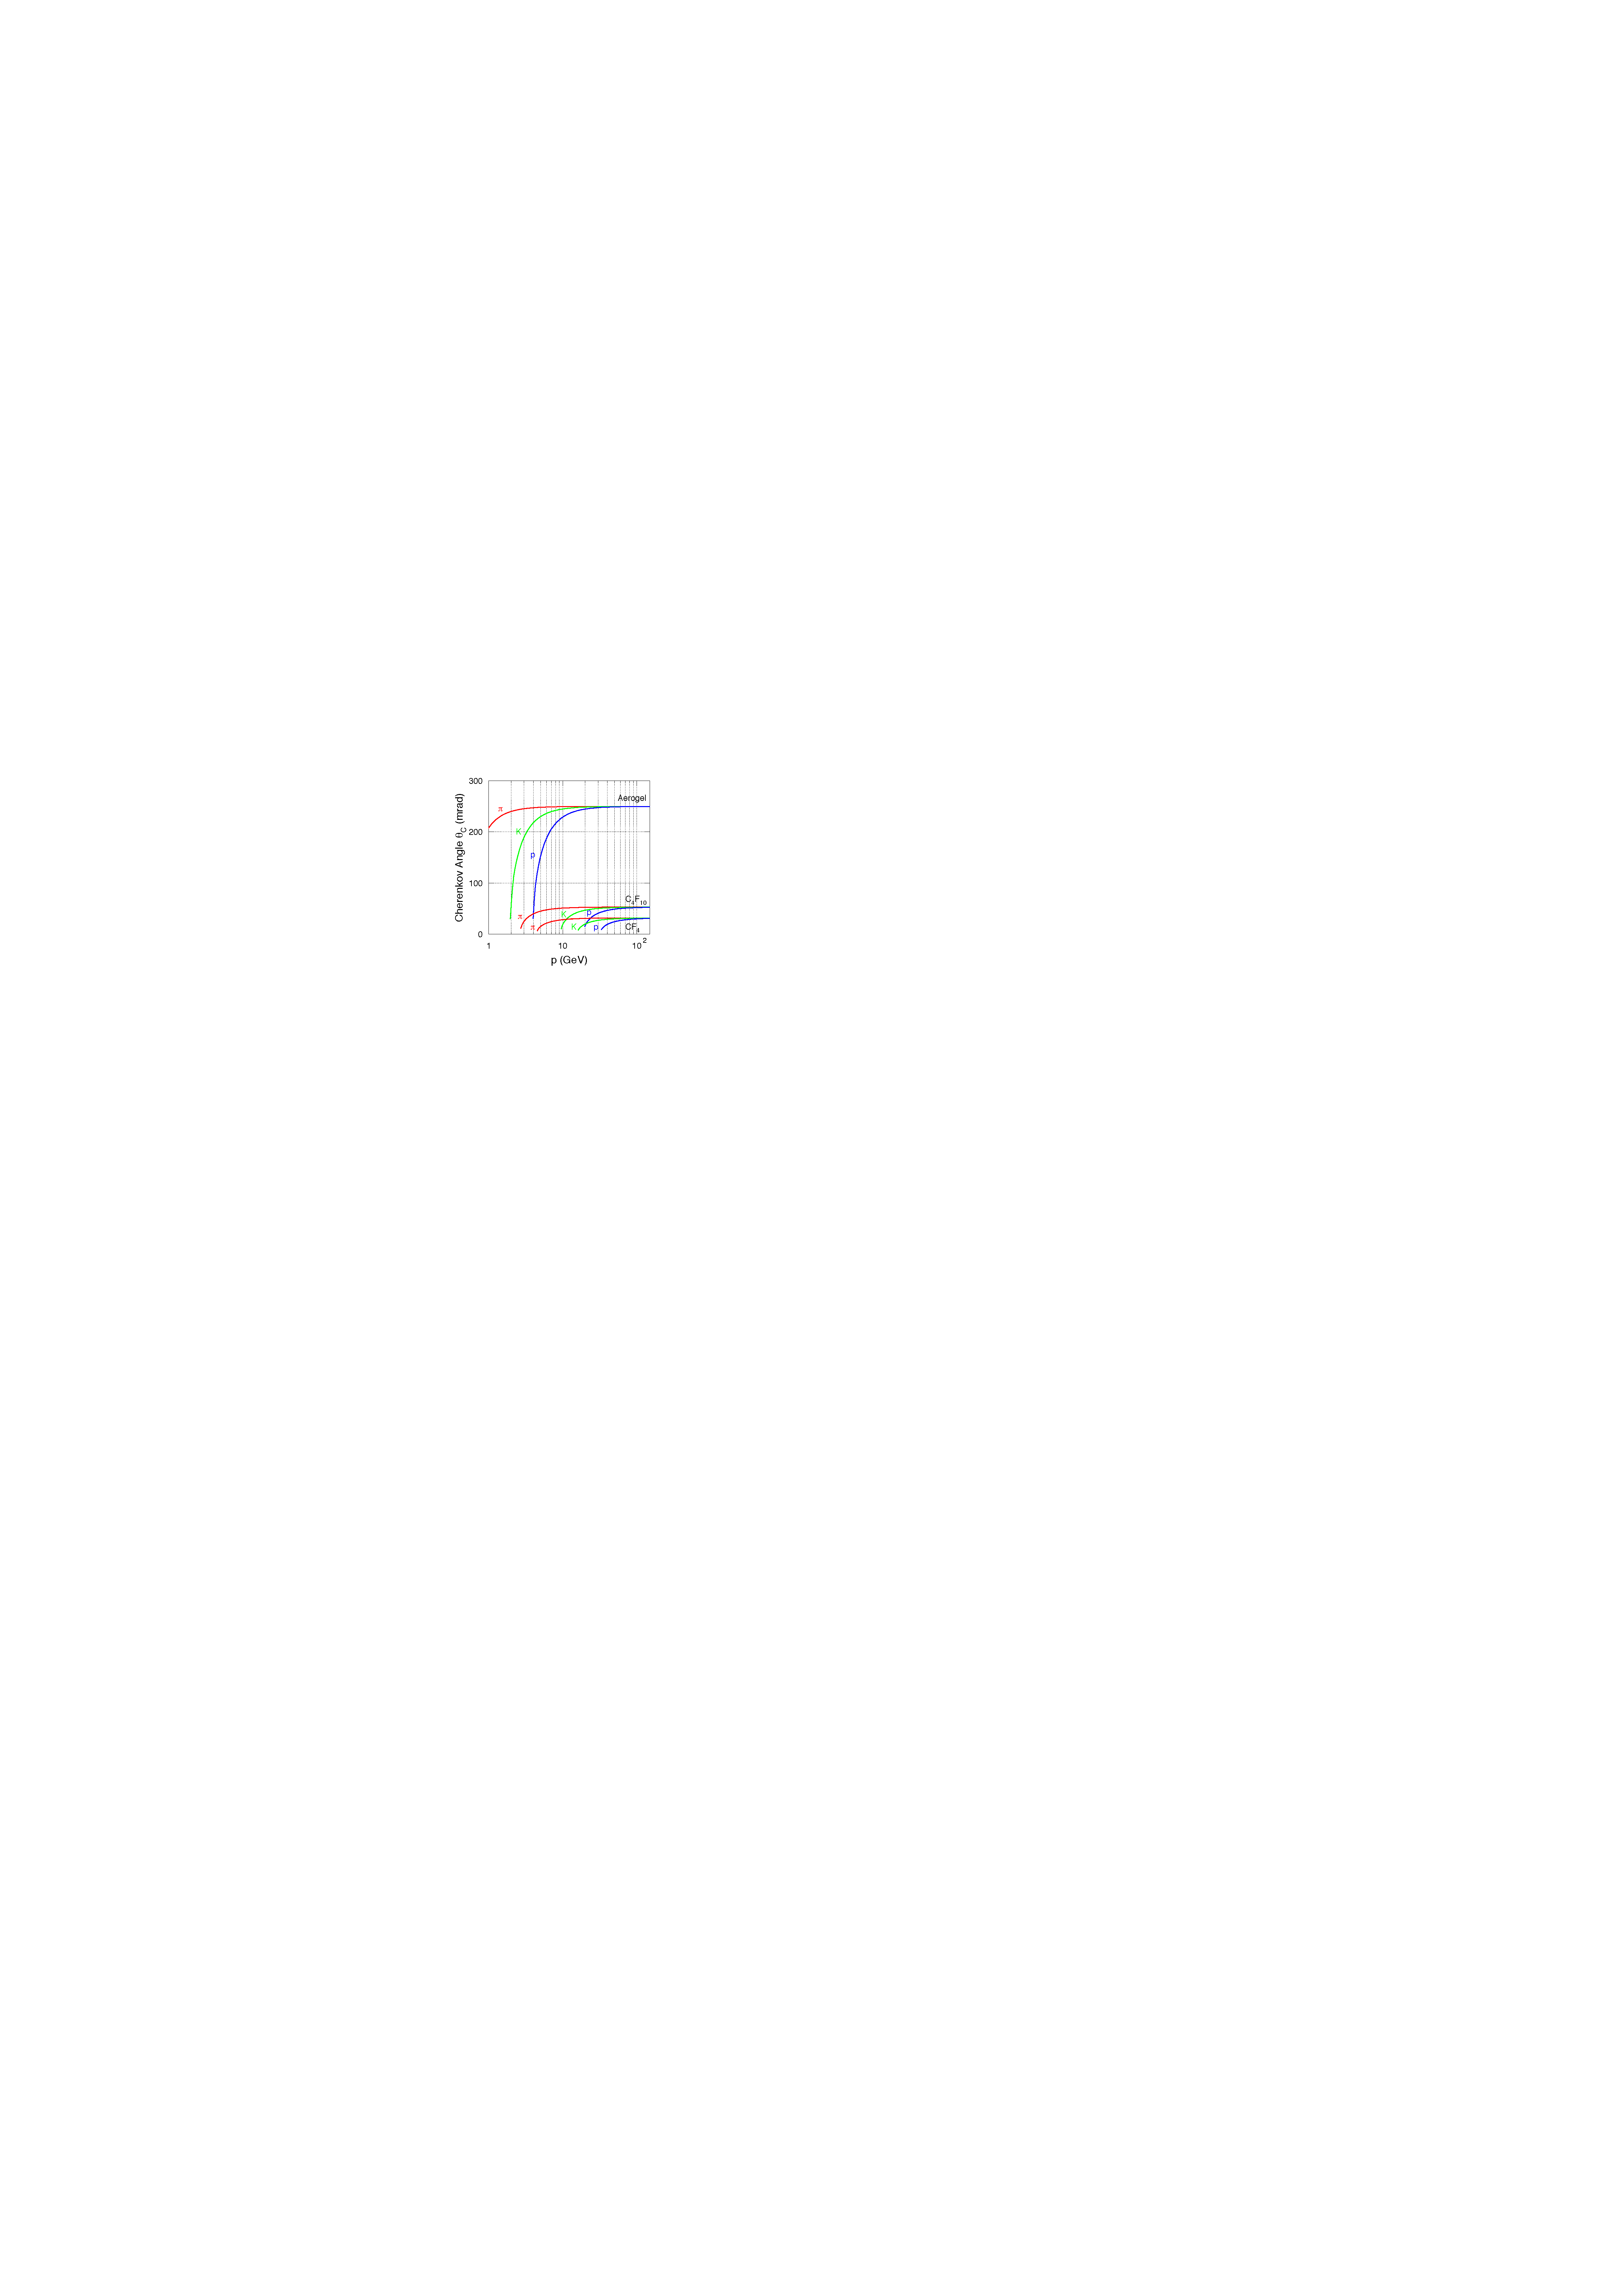
\includegraphics[width=\textwidth]{introduction/cherenkov_angles}
  \caption{%
    Cherenkov angles for different particle species as a function of particle 
    momentum, in the different radiators used in the \rich\ detectors.
    The Cherenkov angle resolution in \richone~(aerogel and \ce{C4F10} 
    radiators) is around \SI{1.6}{\milli\radian}, and around 
    \SI{0.66}{\milli\radian} in \richtwo~(\ce{CF4}).
  }
  \label{fig:intro:lhcb:cherenkov_angles}
\end{figure}

\subsection{Calorimetry}
\label{chap:intro:lhcb:detector:calo}

Given the momentum measurements from the tracking system and the mass 
measurements from the \ac{RICH} detectors, the particle energy is already 
determined.
For hadrons then, a precise calorimetry system is not necessary.
However, the momentum and mass measurements are complex and require a 
significant amount of time to compute, and so cannot be used in the first stage 
of the trigger where the proton-proton collision rate must be reduced from 
\SI{40}{\mega\hertz} down to around \SI{1}{\mega\hertz}.
In addition, the \rich\ detectors are much less sensitive to electron \ac{PID} 
than (\Ppi, \PK, \Pproton), and the tracking system cannot detect photons or 
neutral pions, and so additional detection methods are required.

To provide a fast positive trigger decision for events containing hadronic 
decays of heavy flavour, a hadronic calorimeter, the \hcal, is employed.
This is a sampling calorimeter, composed of alternating layers of iron and 
active scintillating material and positioned downstream of \richtwo.
Hadrons traversing the \hcal\ deposit energy in these layers, with the 
scintillation light collected by wavelength-shifting optical fibres and 
recorded by photo-multiplier tubes.
This general construction and detection mechanism is common to all \lhcb\ 
calorimeters.
The \hcal\ is segmented transversely into square cells, \SI{130}{\milli\metre} 
in width near the beam and \SI{260}{\milli\metre} in width in the outer 
regions, decreasing in granularity to account for the lower particle 
multiplicities.
In the first level trigger, the total transverse energy \ET\ in all clusters of 
$2\times2$ cells is computed, and a positive trigger decision is made if the 
maximum \ET\ is above some threshold, typically between 
\SIrange{3.5}{3.7}{\GeV}.
The \hcal\ provides the highest rate of positive trigger decisions out of those 
at the first trigger level, giving a signal efficiency of around 
\SI{40}{\percent} for two-body \PB decays, and \SI{20}{\percent} for four-body 
\PD decays.
The resolution on the energy measured by the \hcal\ has been measured to be 
$\unc{E}/E = \SI{69 \pm 5}{\percent}/\sqrt{E}$ plus a constant term of \SI{9 
  \pm 2}{\percent}~\cite{Perret:2015pla}.

An electromagnetic calorimeter, the \ecal, is located in front of the \hcal, 
and measures the energies of electrons and photons.
It is segmented in the transverse plane into three regions, increasing in 
granularity towards the beam.
The \ecal\ is partitioned more finely than the \hcal\ due to the smaller 
characteristic scale at which electromagnetic showers occur in comparison to 
hadronic showers.
The energy measurements it makes are used in the first trigger level to accept 
high \ET\ electrons and photons, and in the reconstruction of \Ppizero and 
\Peta mesons offline.
The ability to discriminate between electrons and photons in the trigger 
decision is provided by the scintillating pad/preshower detector~(\spd/\ps) 
which consists of two layers of near-identical scintillator either side of a 
\SI{15}{\milli\metre}-thick layer of lead~(\ce{Pb}) converter, transversely 
segmented in the same manner as the \ecal.
A positive electron trigger decision requires an \ET\ measurement of between 
\SIrange{2.5}{3.0}{\GeV} in a cluster of $2\times2$ cells in the \ecal, along 
with hits in both the \spd\ and the \ps\ pads in front of the corresponding 
\ecal\ cluster.  A positive photon trigger decision is near-identical to this, 
except that no hits must be present in the corresponding \spd\ cells.
The resolution on \ecal\ energy measurements are $\unc{E}/E = \SI{9 \pm 
  0.5}{\percent}/\sqrt{E}$, plus a constant term of 
\SI{0.8}{\percent}~\cite{Perret:2015pla}.

\subsection{Muon reconstruction and identification}
\label{chap:intro:lhcb:muon}

Most particles not absorbed by the calorimeters are muons, and to confirm this 
hypothesis a series of five muon stations, M1--5, are used.
M1 is positioned before the \spd/\ps, and M2--5 are after the \hcal, 
interleaved with \SI{80}{\centi\metre}-thick layers of iron in order to isolate 
high-momentum muons.
For almost all regions across the stations, multi-wire proportional chambers 
are used to collect hits, with the exception being the very inner 
$20\times\SI{24}{\centi\metre\squared}$ region of M1 which uses triple-layered 
gas electron multiplier~(GEM) detectors.
Each station is partitioned into four regions of increasing transverse 
granularity closer to the beam pipe.

A muon momentum of at least \SI{6}{\GeVc} is required for a full traversal of 
all five stations.
Hits recorded in the muon stations are used to provide by \pT\ measurements 
used in the first trigger state, where a track segment must be formed using 
hits in all stations.
The single muon decision requires a segement \pT\ in the range 
\SIrange{1.48}{1.76}{\GeVc}, and the di-muon requires a $\pT^{2}$ in 
\SIrange{1.69}{2.56}{(\GeVc)\squared}.

\section{Online event reconstruction and selection}
\label{chap:intro:lhcb:trigger}

There are three stages to the \lhcb\ trigger system, run sequentially one after 
the other.
Within each stage runs a series of parallel trigger \emph{lines}, and each 
stage runs only if at least one line in the previous stage gave a positive 
decision.

The first stage is a hardware trigger, called the level-zero or \lzero.
It comprises a set of decision units as custom circuitry that evaluate 
decisions at the full \SI{40}{\mega\hertz} of \pp\ collisions provided by the 
accelerator.
The \lzero\ output rate is limited to the \SI{1}{\mega\hertz} rate at which the 
full detector is able to be read out.
The muon stations and the calorimeters can be read at \SI{40}{\mega\hertz}, and 
it is the information from these sub-detectors that is used for making \lzero\ 
decisions.
The single muon decision requires a high \pT\ muon, and the di-muon decision 
requires two.
The hadron, electron, and photon triggers require high \ET\ signatures in the 
\hcal\ or \ecal, as appropriate.
On a positive \lzero\ decision, when one or more line has `fired', the entire 
detector is read out and sent to the \ac{HLT} computing farm for processing in 
software.
Since 2012, around \SI{20}{\percent} of events sent to the farm are deferred to 
disk, to be processed during the inter-fill periods when the detector is 
idle~\cite{1742-6596-513-1-012006}.
This technique increases the average CPU time available for processing each 
event, allowing for looser momentum requirements in the reconstruction and 
hence more efficient triggers.

The first stage of the software trigger, \hltone, and performs a simplified 
track reconstruction in order to confirm the \lzero\ decisions and improve 
their discriminatory power.
Segments in the \velo\ detector are first reconstructed, and \pp\ vertices are 
formed.
Segments that do not have a significant \ac{IP} with respect to all \acp{PV} or 
that cannot be matched to hits in the muon stations are discarded.
The remaining segments are matched to hits in the T-stations to form long 
tracks.
To save processing some due to combinatorics, a search window is defined by a 
minimum momentum that varied between \SIrange{3}{6}{\GeVc} and a minimum \pT\ 
requirement that varied between \SIrange{0.5}{1.25}{\GeVc}.
The transverse momentum window is not required on tracks that can be matched to 
hits in the muon stations.
Using the faster track reconstruction, the mass resolution on \JpsiTomumu\ 
candidates is around \SI{3}{\percent} lower than that achieved in the offline 
reconstruction.

For final states not containing leptons, the most efficient trigger path is 
through the one-track line, which requires the presence of a single, good 
quality, high \pT\ track with a large \ac{IP}.
Typical thresholds were $1.6$--\SI{1.7}{\GeVc} in \pT\ and 
\SI{0.1}{\milli\metre} in \ac{IP}.
This line dominates the \hltone\ output rate, contributing over 
\SI{70}{\percent} of all triggers.
Similar lines exist for muon and di-muon candidates, where the corresponding 
\ac{IP} thresholds are not required if the candidate has a very \pT\ (or a high 
$\Pmuon\APmuon$ invariant mass in the case of the di-muon line).
The muon triggers have efficiencies upwards of \SI{70}{\percent} for \PB\ 
decays containing muons.

Events passing \hltone\ are sent to the second software stage, \hlttwo, at a 
rate of \SI{80}{\kilo\hertz}, where a full event reconstruction is performed, 
including the tracks, vertices, and \ac{PID} information.
As more processing time is now available per event, all \velo\ segments are 
reconstructed as long tracks, with looser search window requirements of $\ptot 
> \SI{3}{\GeVc}$ and $\pT > \SI{0.3}{\GeVc}$, in comparison with \hltone.
A relative loss in efficiency of \SIrange{1}{2}{\percent} per track is seen 
compared to the offline reconstruction.
In \hlttwo, tracks are combined into vertex candidates, and \hlttwo\ lines are 
grouped as either \emph{exclusive}, where decays are fully reconstructed, or 
\emph{inclusive}, where generic signatures are considered.

For beauty decays, the inclusive `topological' lines select two, three, and 
four-body vertices of charged tracks that are characteristic of those produced 
by \PB hadrons.
Input tracks are required to have a high \ac{IP}, and then the resulting vertex 
is selected based on its distance from the \ac{PV}, the \ac{IP} of the vertex 
momentum vector, the \ac{DOCA} and the sum of the \pT\ of the input tracks, and 
the vertex mass and corrected mass, the latter of which accounts for decay 
products not explicitly included in the vertex.
The \ac{DOCA} requirements are loose enough to accommodate \PB decays involving 
a long-lived charm hadron, where a tertiary vertex would be defined in the 
offline reconstruction.
The vertex quantities are used as input to a \ac{BDT}, and the single output 
value is used to make the trigger 
decision~\cite{Gligorov:2011qxa,Gligorov:1384380}.
Decision trees will be discussed in more detail in 
\cref{chap:cpv:kinematic_weighting:bdt_theory}.
A similar set of topological lines exists that are optimised for \PB decays 
that included a high \pT\ muon, and an inclusive \PDstarp\ line exists for 
selecting \DstToDzpi\ with $\decay{\PDzero}{hhX}$ decays, where $hh$ are two 
charged hadrons.
The topological \PB triggers are around \SI{75}{\percent} efficient on average 
at selecting fully charged \PB decays, and the inclusive \PDstarp\ trigger is 
between \SIrange{25}{90}{\percent} efficient.
The efficiencies generally increase with increasing heavy flavour \pT, and for 
the charm triggers are strongly dependent on the multiplicity of the final 
state, with higher multiplicities having a lower efficiency.
The remaining inclusive lines are the single muon and di-muon lines, which are 
similar to those in \hltone.

Exclusive \hlttwo\ lines fully reconstruct the signal decay under study, such 
as \decay{\PB}{\pimpip} and \decay{\PLambdac}{\Pproton\PKminus\Ppiplus}.
Some of these lines are included to increase the efficiency of the inclusive 
lines for specific final states, whilst others are the only trigger path which 
would give a high efficiency trigger path.

After the \acl{HLT}, events passing at least one \hlttwo\ line are saved to 
disk.
The offline processing then begins with the full event reconstruction, which is 
more precise than that in the trigger due to the longer processing times 
permitted.
This is exploited in, for example, the reconstruction of long tracks, where two 
methods are employed offline rather than the one online.
The differences between the online and offline reconstruction were removed 
during \ac{LS1}, which shall be discussed in the following 
\namecref{chap:intro:lhcb:offline}.

\section{Offline data flow and the \ac{LS1} upgrades}
\label{chap:intro:lhcb:offline}

During \runone, all data passing \hlttwo\ was saved to disk and was 
reconstructed offline by a separate software application.
The output of this reconstruction is tracks and the information associated to 
them such as the \ac{DLL} \ac{PID} responses.

To facilitate easier processing offline for analysts, a central selection is 
run called the `stripping', which defines stripping lines that reconstruct 
inclusive and exclusive decays in a similar manner to those defined in \hlttwo.
The lines are grouped into `streams' which group together stripping lines with 
similar selections, such as those of semileptonic \PB decays or di-muon decays.
This is simpler for analysts as they do not need to analyse the entire dataset, 
but only the particular stream that contains the decay are interested in.
Additionally, it saves computing resources as analysts do not need to run the 
candidate building step if they want to add information to their analysis 
later.
In general, any one stripping line contains events which could have been saved 
due to the decision of any trigger line, and so analysts were able to choose 
which triggers to include in their analysis dataset offline.
This can be a complex procedure, as now there are at least two sets of 
selections to consider, those in the trigger and those in the stripping, and 
one must also consider the difference in resolution between the two 
reconstructions: using the same selection online and offline would result in 
visible resolution effects around the selection boundaries, which can be hard 
to model.

To overcome these complications, three parallel efforts were made during 
\ac{LS1}.
The first of these was a major review of the online and offline reconstruction 
software, resulting in a large decrease in the execution time required per 
event in the offline reconstruction, such that the online reconstruction was 
made to be identical to that offline.
The second effort was the development and deployment of a real-time alignment 
and calibration of the full detector per fill.
The full output of \hltone\ is buffered to a \SI{10}{\peta\byte} disk farm, the 
detector alignment and calibration constants are computed using that data, and 
are then applied during the reconstruction performed in 
\hlttwo~\cite{Dujany:082010}.
The \hlttwo\ processing is then fully asynchronous to the \ac{LHC}.
The third effort, facilitated by those previous, was the introduction of the 
Turbo stream processing model~\cite{Benson:2019752}.
Given that the additional offline processing was no longer necessary to improve 
the resolution of the various physics quantities, and that the best possible 
detector alignment and calibration is already applied, it was realised that 
physics analyses could be performed directly on the output of the trigger.

There are several benefits due to \ac{LS1} efforts.
The improvement of the online reconstruction allows for parity between the 
online and offline selections, increasing the trigger efficiency, the possible 
number of signal candidates available for analysis, and the total processing 
time required.
This in turn allowed for the inclusion of a new two-track trigger in \hltone, 
which is able to build and select two-prong vertices, further increasing 
efficiency.
In addition, these efforts negate the need for an additional, offline 
reconstruction, saving computing resources,
 allowing analyses and data quality reports to progress more quickly as the 
 data are made available almost immediately, within hours rather than the days 
 or weeks with the \runone\ processing model.
 Analyses have already been performed that exploited this 
 model~\cite{LHCb-PAPER-2015-037,Aaij:2015bpa}.

 The Turbo stream currently has some limitations, however.
 The most restrictive of these is that the candidates available to analysts are 
 only those explicitly used in the trigger decision.
 For example, if a trigger line reconstructs \DzToKpi\ and the candidate passes 
 the selection, analysts can only use the information pertaining to the kaon 
 and pion tracks, the \PDzero vertex, and the associated primary vertex.
 For many analyses, this information is all that is needed, however sometimes 
 additional information about the event is required.
 Effort is ongoing to resolve these problems, and it is expected that a vast 
 majority of analyses will be using the Turbo stream in \runthree.

\section{Simulation}
\label{chap:intro:lhcb:simulation}

Simulated data is used to model effects that cannot be modelled using the real 
data, such as acceptance efficiencies, and to perform detector performance 
studies during design phases.

Proton-proton collisions are generated by the \pythia\ 8 program using a tune 
specific to \lhcb.
\pythia\ simulates the parton interactions, quark and gluon fragmentation, and 
resulting hadronisation and creation of other particles, such as leptons.
The behaviour of the hadrons is simulated by the \evtgen\ program, which models 
phenomena such as branching fractions, neutral meson mixing, \CP\ violation, 
decay amplitude models, and decay times.
Simulated samples for a specific decay are generated by running \pythia\ in 
`minimum bias mode', where proton-proton collisions are generated until the 
head of the decay is created somewhere in the set of particles produced, and 
then this head particle is forced to decay to the final state under study by 
\evtgen~\cite{Clemencic:2011zza}.
The behaviour of the other particles generated in the event is also controlled 
by \evtgen, but is not forced to any particular state.

The total simulation is configured to model the beam parameters relating to the 
`real data' the \ac{MC} is to be used with~\cite{Belyaev:1322400}.
After \evtgen, the particles are propagated through a simulation of the entire 
detector using the \geant\ 4 program, where interactions with the detector are 
recorded as `\ac{MC} hits'.
These \ac{MC} hits are converted into a format mimicking the electrical 
response of the real detector through an \lhcb-specific emulation, and the 
response is processed through the trigger and reconstruction software in an 
near-identical manner to real data.
The \lzero\ trigger decisions are emulated in software, and the trigger 
configuration used for a given data-taking year, such as 2011, is chosen to be 
the one that is most representative.

The simulated data is processed in such a way that reconstructed objects can be 
associated to the \ac{MC} objects that created them.
For charged, stable particles reconstructed via tracks, a particle is 
associated to an \ac{MC} particle if at least \SI{70}{\percent} of the hits 
comprising the associated track were deposited by the \ac{MC} particle in 
question.
The process of assigning \ac{MC} objects to reconstructed objects is referred 
to as truth matching.
Tracks are classified as `ghost' tracks if there are no \ac{MC} particles that 
can be associated to them.
Vertices can then be assigned categories based on the associations of their 
input tracks.
A `signal vertex' is defined as one in which all inputs are associated to 
\ac{MC} particles, all inputs have been assigned a particle identity equal to 
that of their associated \ac{MC} particle, all inputs have been associated with 
\ac{MC} particles which come from the same true \ac{MC} parent, and the 
identity of the \ac{MC} parent matches that assigned to the vertex.
Any deviation from these requirements results in the vertex being assigned a 
particular \emph{background category}, dependent on the nature of the 
deviations~\cite{Gligorov:1035682}.
For example, if at least one track is a ghost, the vertex is classified as a 
ghost, and if at least one track is associated to an \ac{MC} particle with a 
different \ac{PID}, the vertex is classified as a misidentification.
In the case of a vertex than can be associated to an \ac{MC} particle, the 
vertex can be further classified as prompt or secondary based on the true 
lifetime of the \ac{MC} particle.
For consistency of terminology, signal vertices are referred to as having a 
`background category' of `signal'.

In general, separate samples of simulated data are produced on a per-analysis 
basis, with independent samples generated for different beam energies and 
dipole magnet polarities (usually only `up' and `down').
The generation of \ac{MC} is done centrally by the experiment using a globally 
distributed network of computers, and the resulting data files are then made 
available to analysts in the same way as for real data, with the additional 
inclusion of the truth-matching information.
